\documentclass[a4paper,12pt]{article}
\usepackage[swedish]{babel}
\usepackage[utf8]{inputenc}
\usepackage{amsmath, amsthm, amssymb}
\usepackage{pgfplots, scrextend, gensymb}
\pgfplotsset{compat=1.18}
% Ändra INTE nästa rad (säger var texten ska typsättas)
\usepackage[a4paper,includeheadfoot,margin=2.54cm]{geometry}
% Ändra INTE nästa rad (som lägger till radnummer till vänster)
\usepackage[left]{lineno}


% Ändra INTE raderna nedan
% Koden är från https://tex.stackexchange.com/questions/43648/
% Den fixar radnumrering av text i närvaro av matematikomgivningar
\newcommand*\patchAmsMathEnvironmentForLineno[1]{%
  \expandafter\let\csname old#1\expandafter\endcsname\csname #1\endcsname
  \expandafter\let\csname oldend#1\expandafter\endcsname\csname end#1\endcsname
  \renewenvironment{#1}%
     {\linenomath\csname old#1\endcsname}%
     {\csname oldend#1\endcsname\endlinenomath}}% 
\newcommand*\patchBothAmsMathEnvironmentsForLineno[1]{%
  \patchAmsMathEnvironmentForLineno{#1}%
  \patchAmsMathEnvironmentForLineno{#1*}}%
\AtBeginDocument{%
\patchBothAmsMathEnvironmentsForLineno{equation}%
\patchBothAmsMathEnvironmentsForLineno{align}%
\patchBothAmsMathEnvironmentsForLineno{flalign}%
\patchBothAmsMathEnvironmentsForLineno{alignat}%
\patchBothAmsMathEnvironmentsForLineno{gather}%
\patchBothAmsMathEnvironmentsForLineno{multline}%
}

% Ändra INTE nästa rad (gör så radnummer skrivs med fet stil)
\renewcommand\linenumberfont{\normalfont\bfseries\small}

\title{Skidbacken}
%
\author{Zacharias Brohn\thanks{email:
        \texttt{zacbro-8@student.ltu.se}}\\  
        ~ \\
        Luleå tekniska universitet \\ 
        971 87 Luleå, Sverige}
%          
\date{\today}

\begin{document}

\linenumbers % ger radnumrering

\maketitle

\begin{abstract}
  I denna rapport ska jag beskriva och förklara uppgifter angående en given funktion på en kurva 
\end{abstract}
\section{Introduktion}
\label{sec:introduktion}
Rapporten kommer lösa och beskriva uppgifter kring en skidbacke som har fallhöjden 500 meter. Här ser du den grafiskt ritad:

\noindent
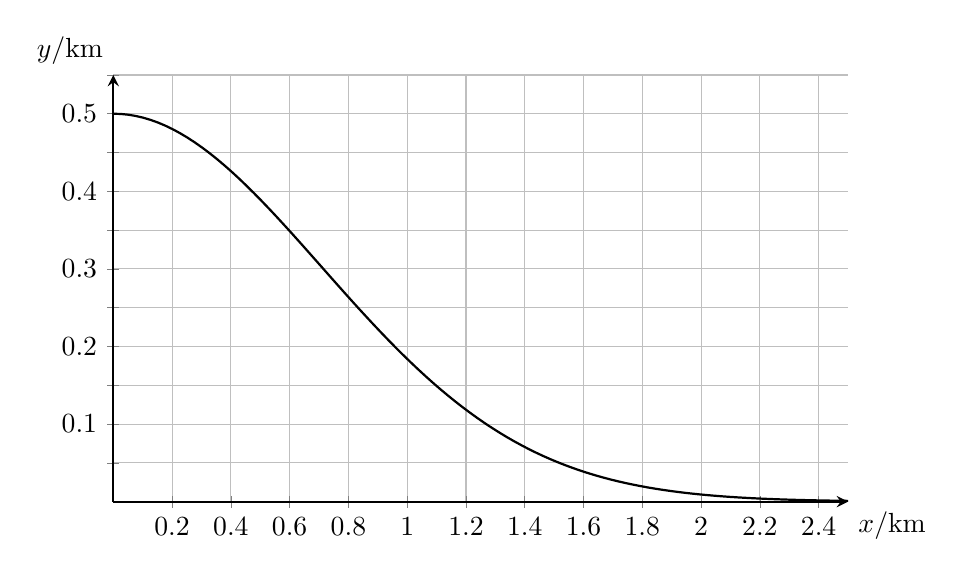
\begin{tikzpicture}
  \begin{axis}[
      width=0.9\linewidth,
      height=7cm,
      %axis tick,  % Equal scaling on both axes
      axis lines=middle, % Draw the axes in the middle with arrows
      xlabel={$x$/km},
      ylabel={$y$/km},
      domain=0:2.5,      % Set the range for x-axis
      samples=100,       % Set the number of samples for smoothness
      xmin=0,            % Start x-axis from 0
      ymin=0,            % Start y-axis from 0
      xmax=2.5,          % Limit x-axis to 2.5 for matching graph
      ymax=0.55,          % Limit y-axis to 0.5
      grid=major,        % Major grid only
      thick,             % Thicker lines
      every axis x label/.style={at={(current axis.right of origin)}, anchor=north west},
      every  axis y label/.style={at={(current axis.above origin)}, anchor=south east},
      xtick={0,0.2,...,2.5},  % Define x-tick steps
      ytick={0,0.05,0.1,...,0.6},  % Define y-tick steps
      yticklabels={0.0,,0.1,,0.2,,0.3,,0.4,,0.5,,0.6}
  ]
      \addplot[black] {0.5*exp(-x^2)};
  \end{axis}
\end{tikzpicture}\newline
Grafen är ritad med ett samband mellan y (höjden i km.) och x (längden i km.) som kan srivas som:\\
$y = 0,5e^{-x^2}$ $\>$ $\>$ där $\>$ $\>$ $0 \leq x \leq 2,5$\\
\section{The angle of a slope}
\label{sec:uppg1}
  First we solve:\\
  \begin{addmargin}[1em]{1em}
    Determine the angle at which the curve of the function is inclined at the point $x=0,8$.\\
  \end{addmargin}
  To do this, we first need to calculate the derivative $\left(\frac{dy}{dx}\right)$ of the function, which will give us the slope of the tangent line at that point. From the slope, we can then calculate the angle using the arctangent function. Because the function involves an exponential expression, we will use the \textbf{chain rule}:
  \subsection{Splitting the function}
  The function $y=0,5e^{-x^2}$ can be viewed as a composition of two functions:
  \begin{itemize}
    \item The outer function $f(u)=0,5e^u$, where $u=-x^2$.
    \item The inner function $g(x)=-x^2$.
  \end{itemize}
  According to the chain rule, the derivative of the composite function is:
  \begin{displaymath}
    \frac{dy}{dx} = \frac{dy}{du} \cdot \frac{du}{dx}
  \end{displaymath}
  \subsection{Step~1: Derivative of the Outer Function}
  First, we differentiate the outer function $y = 0,5e^u$ with respect to $u$. The derivative of $e^u$ with respect to $u$ is simply $e^u$, and since there is a constant 0,5 in front, we have:
  \begin{equation}
    \frac{dy}{du} = 0,5e^u
  \end{equation}
  \subsection{Step~2: Derivative of the Inner Function}
  Next, we differentiate the inner function $u = -x^2$ with respect to $x$ using the basic power rule differentiation:
  \begin{equation}
    \frac{du}{dx} = \frac{d}{dx}\left(-x^2\right) = -2x
  \end{equation}
  \subsection{Step~3: Applying the Chain Rule}
  Now, we apply the chain rule by multiplying the results from Step~1 and Step~2:
  \begin{equation}
    \frac{dy}{dx} = \frac{dy}{du} \cdot \frac{du}{dx} = 0,5e^{-x^2} \cdot \left(-2x\right)
  \end{equation}
  And by simplifying this expression we get:
  \begin{equation}
    \frac{dy}{dx} = -x \cdot e^{-x^2}
  \end{equation}
  Thus we have the derivative of $y$.
  \subsection{Finding the Slope at $x = 0,8$}
  Now that we have the general expression for the derivative, we can calculate the slope of the curve at the point $x$. Substituting $x = 0,8$ into the derivative as well as simplifying:
  \begin{equation}
    \begin{split}
      y'(0,8) & = -0,8 \cdot e^{-\left(0,8\right)^2} \\
              & = -0,8 \cdot e^{-\left(0,64\right)} \\
              & \approx -0,8 \cdot 0,5272 \approx -0,42
    \end{split}
  \end{equation}
  So the answer is that the slope of the tangent line at $x = 0,8$ is approximately $-0,42$.
\section{Second derivative}
\label{sec:uppg2}
Here our task is:\\
\begin{addmargin}[1em]{1em}
  Find an equation where the angle is the steepest using this function:
  \begin{displaymath}
    y = 0,5e^{-ax^2}
  \end{displaymath}
\end{addmargin}
Where $a$ is a constant and $x$ is in the range $0 \leq x \leq 2,5$. The second derivative will tell us how the slope of the curve is changing and will let us analyze the concavity of the function. But first, we need to calculate the first derivative $y'$.
\subsection{First Derivative}
Just like earlier we will make use of the \textbf{chain rule} for this, so, again:
\begin{itemize}
  \item The outer function is $f(u) = 0.5e^u$, where $u = -ax^2$
  \item The inner function is $g(x) = -ax^2$.
\end{itemize}
The outer function's derivative with respect to $u$ is, once again, $e^u$, so we have:
\begin{equation}
  \frac{dy}{du} = 0,5e^u
\end{equation}
And the inner function's derivative with respect to $x$ using the power rule, we get:
\begin{equation}
  \begin{split}
    \frac{du}{dx} &= \frac{d}{dx}\left(-ax^2\right) \\
                  &= -2ax
  \end{split}
\end{equation}
Now we can apply the chain rule:
\begin{equation}
  \begin{split}
    \frac{dy}{dx} &= \frac{dy}{du} \cdot \frac{du}{dx} \\
                  &= 0,5e^{-ax^2} \cdot \left(-2ax\right)
  \end{split}
\end{equation}
Now that we have the first derivative, we can simplify it:
\begin{displaymath}
  \begin{split}
    y'  &= 0,5e^{-ax^2} \cdot \left(-2ax\right) \\
        &= -ax \cdot e^{-ax^2}
  \end{split}
\end{displaymath}
\subsection{Finding the Second Derivative}
Finally we can work toward finding the Second Derivative $\frac{d^2y}{dx^2}$. To do this we can use the \textbf{product rule} and, once again, the \textbf{chain rule}.
\subsection*{The Product Rule}
The product rule states:
\begin{displaymath}
  \frac{d}{dx}\left(u\left(x\right) \cdot v\left(x\right)\right)
  = u'\left(x\right) \cdot v\left(x\right) + u\left(x\right) \cdot v'\left(x\right)
\end{displaymath}
And in our case:
\begin{itemize}
  \item $u\left(x\right) = -ax$
  \item $v\left(x\right) = e^{-ax^2}$
\end{itemize}
Of which we need to find the derivative for both:
\begin{equation}
  \begin{split}
    u'\left(x\right)  &= -as \\
    v'\left(x\right)  &= e^{-ax^2} \cdot \left(-2ax\right) \\
                      &= -2axe^{-ax^2}
  \end{split}
\end{equation}
Now we need to apply the product rule:
\begin{equation}
  \begin{split}
    \frac{d^2y}{dx^2} &= \frac{d}{dx}\left(u\left(x\right) \cdot 
                         v\left(x\right)\right) \\
                      &= u'\left(x\right) \cdot v\left(x\right) + u\left(x\right) \cdot v'\left(x\right) \\
                      &= \left(-a\right) \cdot e^{-ax2} + \left(-ax\right) \cdot \left(-2axe^{-ax^2}\right)
  \end{split}
\end{equation}
\section{Och ännu nästa (del-) uppgift...}
\label{sec:uppgN}

\section{Diskussion [och slutsatser]}
\label{sec:disk}

Sammanfatta vad som avhandlats i rapporten, vad du kommit fram till,
och sätt det i sitt sammanhang. 
%
\begin{thebibliography}{99}
%
\bibitem{latexcompanion} 
Michel Goossens, Frank Mittelbach, and Alexander Samarin. 
\textit{The \LaTeX\ Companion}. 
Addison-Wesley, Reading, Massachusetts, 1993.
%
\bibitem{einstein} 
Albert Einstein. 
\textit{Zur Elektrodynamik bewegter K{\"o}rper}. (German) 
[\textit{On the electrodynamics of moving bodies}]. 
Annalen der Physik, 322(10):891–921, 1905.
%
\end{thebibliography}
%
\end{document}
